% !TeX root = Dissertation.tex
\chapter{Analyse}

\begin{figure}[h]\centering
\rule{6cm}{4cm}
\caption{Ein schwarzes Viereck}
\end{figure}

\blindtext[10]

\blindtext[10]

\begin{figure}[h] \center
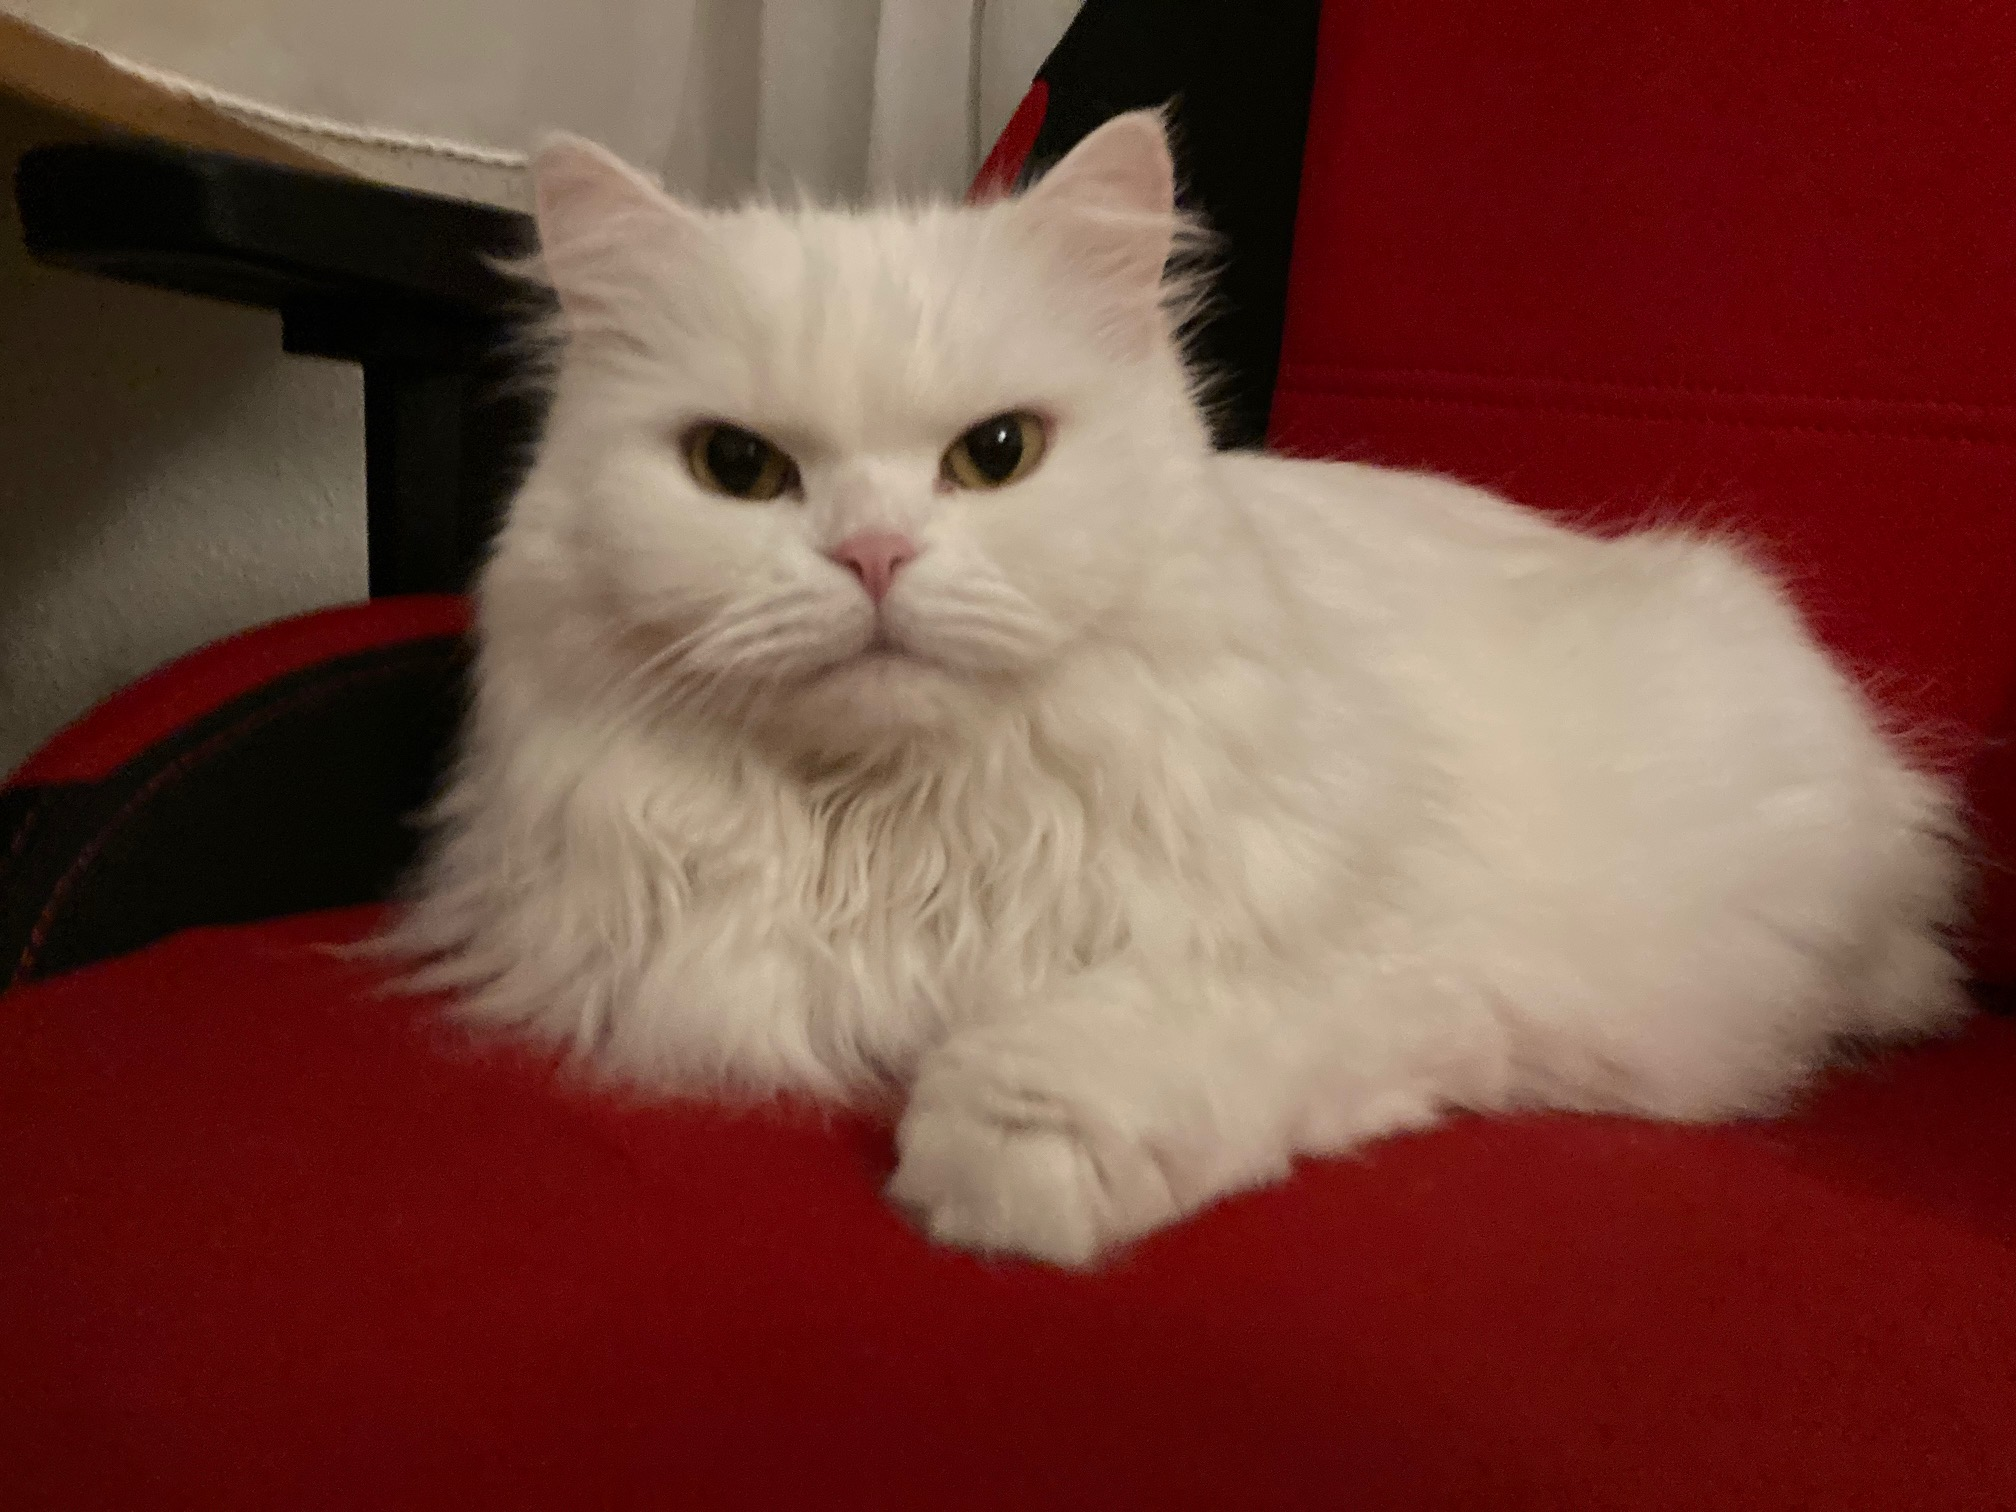
\includegraphics[width=0.8\textwidth]{Images/Katze}
\caption{Meine Miezekatze}\label{fig:Katze1}
\end{figure}


\blindtext[10]

\blindtext[10]

\blindtext[10]

Siehe Abbildung \ref{fig:Katze1}

\blindtext[10]


\begin{figure}[h]\centering
\rule{6cm}{4cm}
\caption{Ein schwarzes Viereck}
\end{figure}

\blindtext[10]

\blindtext[10]

\blindtext[10]

\blindtext[10]

\blindtext[10]



\blindtext[10]


\begin{figure}[h]\centering
\rule{6cm}{4cm}
\caption{Ein schwarzes Viereck}
\end{figure}

\blindtext[10]

\blindtext[10]

\blindtext[10]

\blindtext[10]

\blindtext[10]



\blindtext[10]


\begin{figure}[h]\centering
\rule{6cm}{4cm}
\caption{Ein schwarzes Viereck}
\end{figure}

\blindtext[10]

\blindtext[10]

\blindtext[10]

\blindtext[10]

\blindtext[10]



\blindtext[10]

